\documentclass[11pt]{article}
\usepackage{amsmath, amssymb, amscd, amsthm, amsfonts}
\usepackage{graphicx}
\usepackage{tikz}
\usepackage[]{tikz-3dplot}
\usepackage[colorlinks]{hyperref}
\usepackage[nameinlink,noabbrev]{cleveref}
\usepackage{float}
\usepackage{caption}
\usepackage{subcaption}
\usepackage[a4paper, total={6in, 8in}]{geometry}
\usepackage{soul}
\usepackage{enumitem}   

%\oddsidemargin 40pt
%\evensidemargin 40pt
%\marginparwidth 40pt
%\marginparsep 40pt
\topmargin 0pt
\headsep 0pt
\textheight 8.7in
%\textwidth 6in
\linespread{1.2}

\title{Deep Learning FSS22 \\ Assignment 2: CNNs and RNNs}
\author{Timur Michael Carstensen - 1722194}
\date{08.05.2022}


\newcommand{\rr}{\mathbb{R}}

\DeclareMathOperator*{\argmax}{arg\,max}
\DeclareMathOperator*{\argmin}{arg\,min}

\newcommand{\al}{\alpha}
\DeclareMathOperator{\conv}{conv}
\DeclareMathOperator{\aff}{aff}

\begin{document}

\pagenumbering{roman}

\maketitle


\newpage

\tableofcontents

\newpage


\pagenumbering{arabic}

\section{Convolutional Neural Networks}\label{sec:cnn}

\subsection{a)}\label{subsec:cnn-a}
\begin{enumerate}[label=(\roman*)]
\item \textit{3x3 convolutional layer with bias, 1 input channel, 32 output channels, stride 1, padding 1 on each side} 

Input: 28x28x1\\
Output: 28x28x32\\
No. of Parameters: 32 3x3 kernel matrices and 32 bias terms \\

\item \textit{Logistic activation function}

Input: 28x28x32 \\
Output: 28x28x32 \\
No. of Parameters: none\\

\item \textit{2x2 max-pooling layer with stride 2}

Input: 28x28x32\\
Output: 14x14x32\\
No. of Parameters: none \\

\item Linear layer with 10 hidden units

Input: 14x14x32\\
Output: 10 \\
No. of Parameters: 10x6270=62720 \\

\item Log-softmax function

Input: 10 \\
Output: 10 \\
No. of Parameters: none \\
\end{enumerate}

Interpretation of the outputs: log-probabilities for the 10 different classes of garments.

\subsection{b)}\label{subsec:cnn-b}
Cf. Code.

\subsection{c)}\label{subsec:cnn-c}
Cf. code.
\subsection{d)}\label{subsec:cnn-d}
Cf. Code.
\subsection{e)}\label{subsec:cnn-e}

\begin{figure}[hbt]
  	\center
  	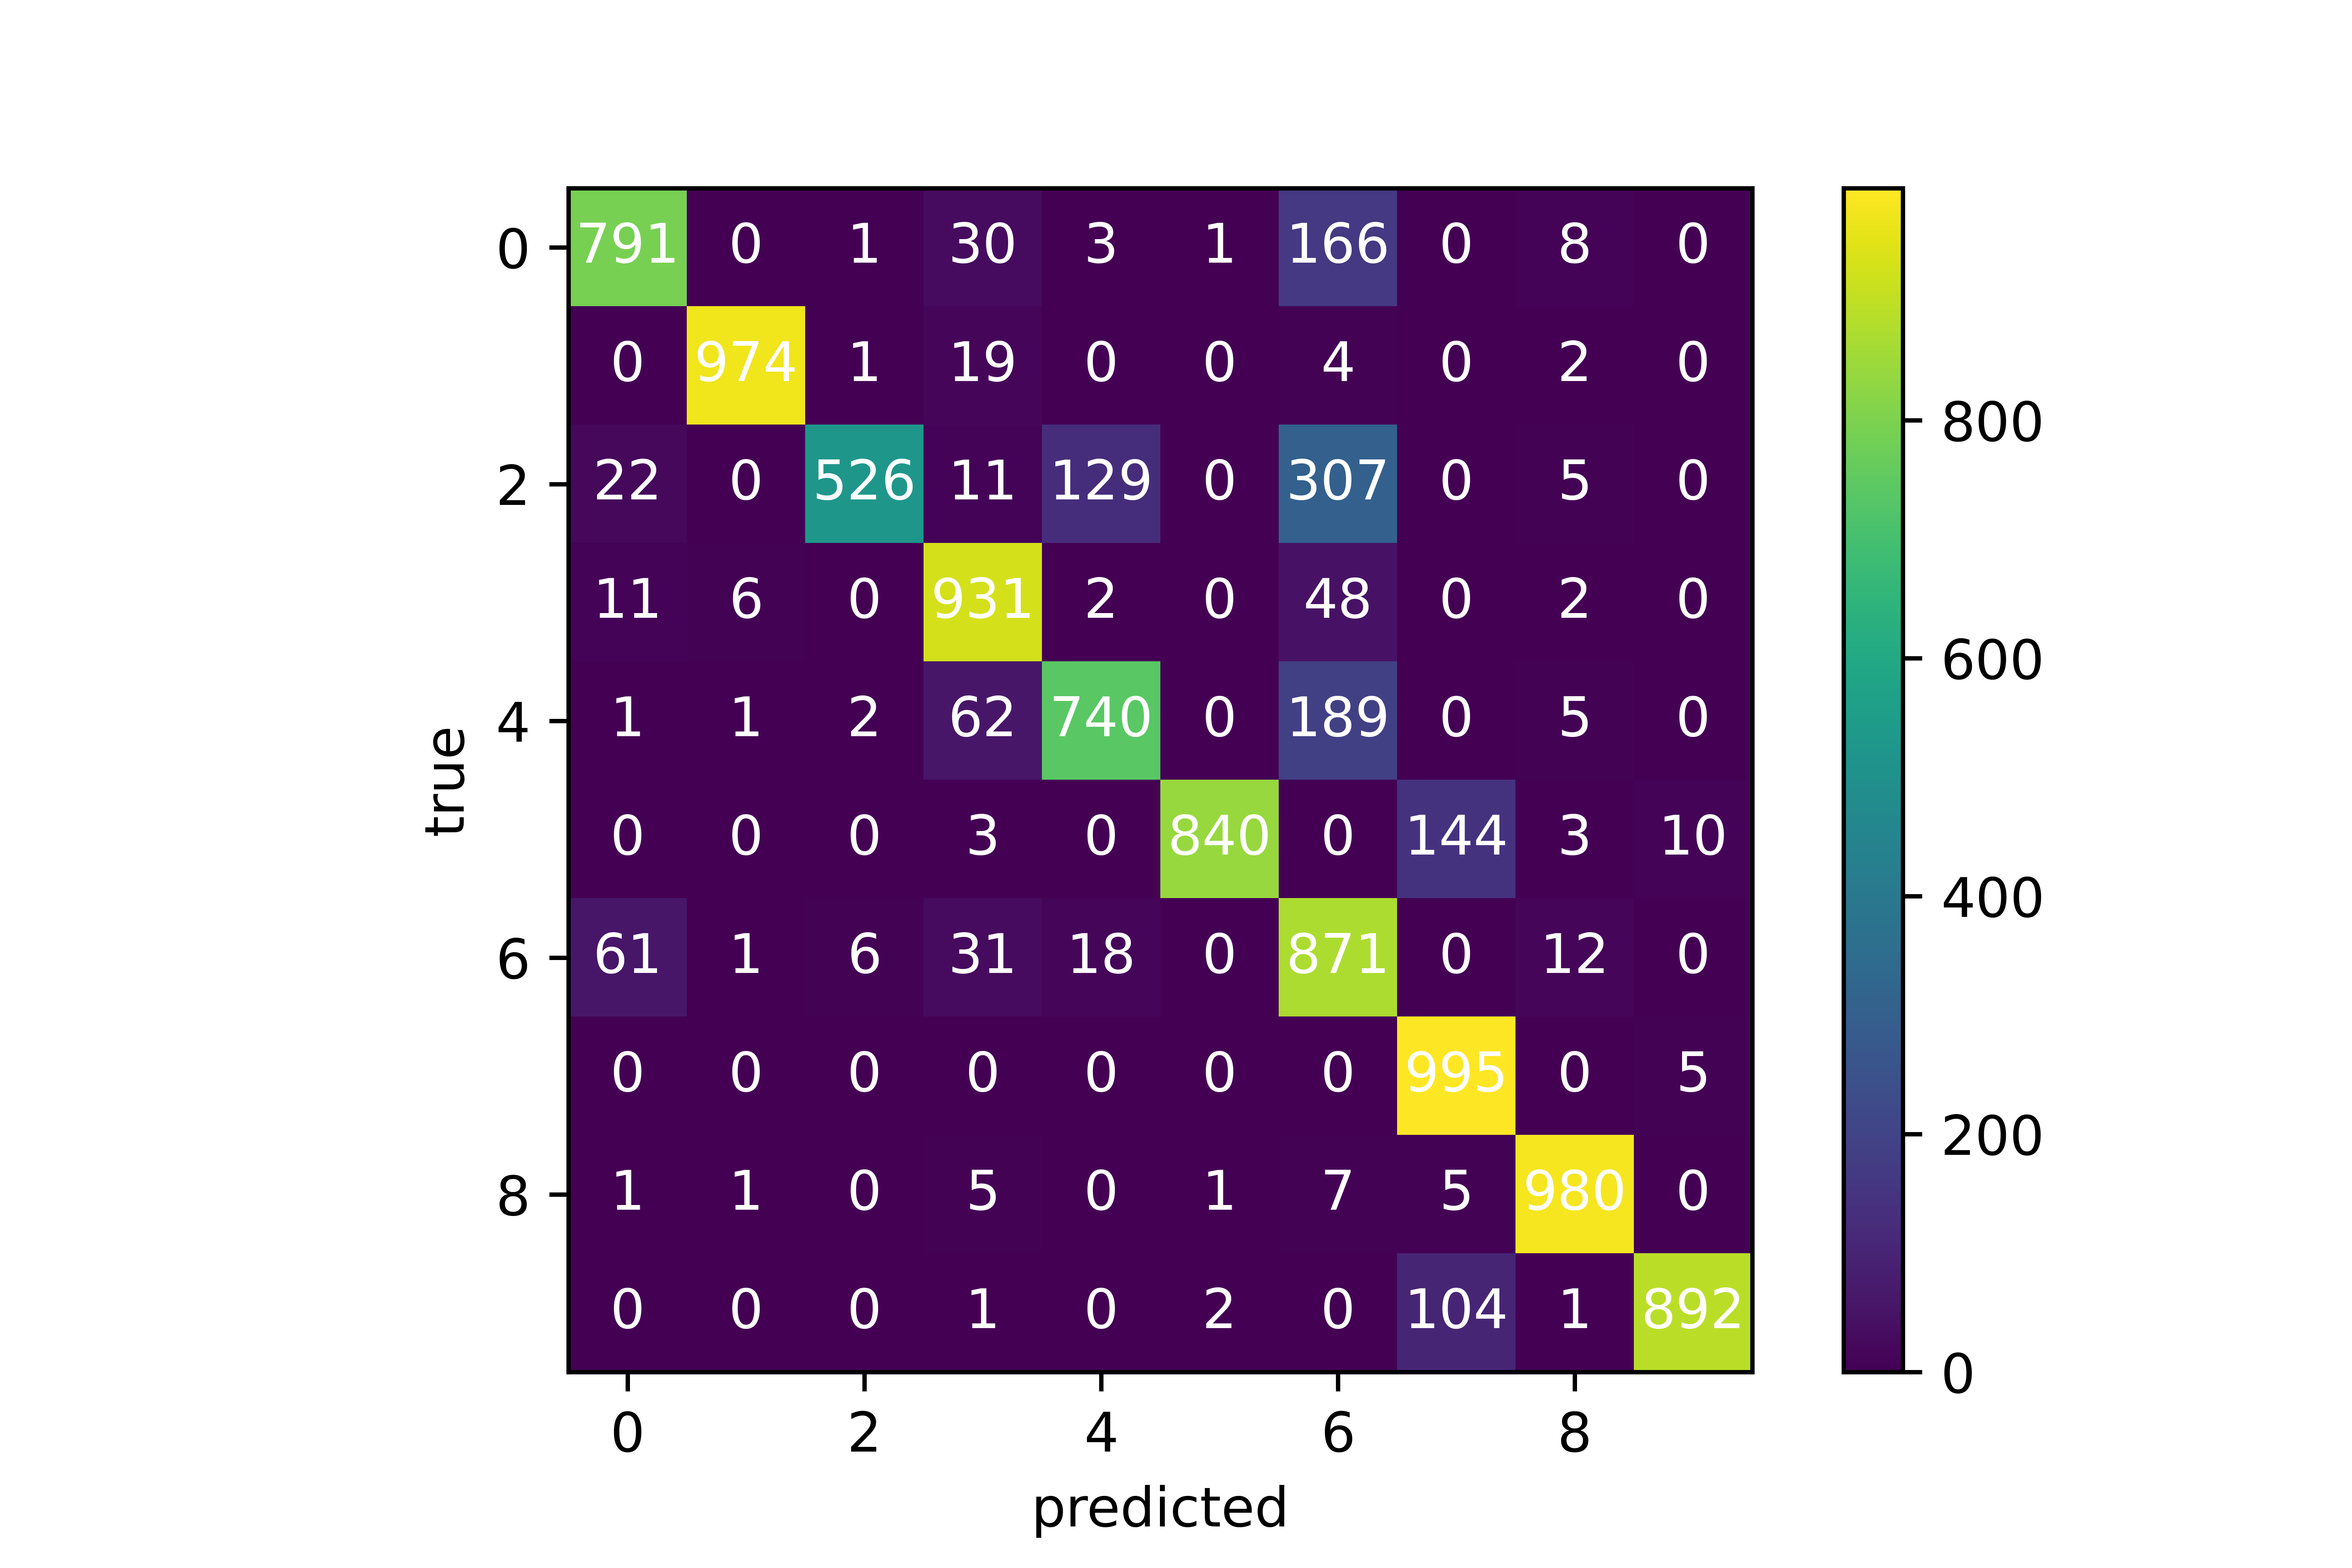
\includegraphics[width=\columnwidth]{assets/conf_mat}
  	\caption{Confusion matrix for the fashion MNIST dataset}
  	\label{fig:f-mnist-conf-mat}
\end{figure}

\noindent The model achieved an accuracy of 87.29\%. When inspecting the individual classes, we can see that the accuracy varies from 99.2\% to as low as 61.6\%. The model performs the worst on pullovers and t-shirts with accuracies of 61.6\% and 75.9\% respectively. It performs best on sneakers and ankle boots with accuracies of 99.2\% and 98.3\% respectively. The rest of the classes are in the 80\% to 90\% range, with bags also performing particularly well (accuracy: 96.7\%). I would expect the model to perform well on unique shapes and make mistakes on garments that are quite similar in shape. That is, shirts and pullovers are easy to confuse since they have similar shapes and sneakers, ankle boots and bags have (very) distinct shapes as compared with the rest of the garments. This is confirmed in \autoref{fig:f-mnist-conf-mat} where we can see that pullovers are often confused for shirts and coats. Our model can discriminate footwear from non-footwear quite well, though it does have issues distinguishing sandals from sneakers occasionally. These mistakes are reasonable for our model to make since it does not learn anything about the actual meaning of what makes a shirt a shirt or a pullover a pullover. 


\subsection{f)}\label{subsec:cnn-f}
Not attempted.

\section{Recurrent Neural Networks and Pretraining}\label{sec:rnn}
\subsection{a)}\label{subsec:rnn-a}
Cf. Code.
\subsection{b)}\label{subsec:rnn-b}
We can see that the error on our training set decreases with each subsequent epoch. That is, for our first batch the average training loss is 0.6865 and for our fifth epoch it is 0.3577. However, at the same time, the average loss on our validation set reaches a minimum at around epoch 4 and starts to slightly increase with epoch 5 (0.6657 vs. 0.6667). This indicates that we are overfitting our model on our training data and not converging to a \textit{global} minimum. I suspect this to be because of our embedding layer which we train on our training data. For tokens not encountered in the training set, the corresponding embeddings retain their random initialisations and thus reduce our model's performance in the forward pass on the validation set. This effect may have been lessened if our vocabulary in the training set were larger or if we had more training examples in general. 


\subsection{c)}\label{subsec:rnn-c}
The GloVe \cite{pennington2014glove} embedding file contains word embeddings for 29841 of the 32362 unique word ids in our dataset. In contrast to before, the embeddings are 100-dimensional vectors containing the representations of our words. The "word-embeddings.txt" file is organised in such a way that each row is a key, value pair with the key being the word id and the value being the embedding $\in\mathbb{R}^{100}$. This way, we can match the embeddings to our corpus with the word ids.

\subsection{d)}\label{subsec:rnn-d}
The first observation that we can make is that the average validation losses of both the RNN with and without finetuning stay constantly below that of the simple RNN. The average training set loss stays above the simple RNN when do not finetune our embeddings and falls below it if we do. The average training loss for the RNN with GloVe embeddings and fine-tuning also decreases much faster than that of the other models. When inspecting the validation loss in the last epoch of the GloVe model with fine-tuning we can see that we are again on an upward trajectory toward the end of the epoch. Hence, we are starting to overfit. The model with GloVe embeddings and without fine-tuning seems to stabilise and converges at an average validation loss of 0.6. We can conjecture that this is the best loss that we can achieve given our embeddings and model design. Better generalisation performance could possibly be achieved by using a larger training set, initialising more (or all) of the word vectors with GloVe embeddings and fine-tuning the model up until we observe an up-tick in validation loss and stop training at that point.

\subsection{e)}\label{subsec:rnn-e}



\bibliographystyle{alpha}
\bibliography{references}

\end{document}
